\section{The theory in more detail}
\label{app:theory}

\paragraph{Reading the barrier.} Two populations with the same attacker can have very different barriers, because $B_\alpha(A)$ depends only on benign traffic. Every additional benign group raises the bar; a campaign that copies benign behaviour lowers its own height. The propositions are standard arguments, stated because they organise the experiments and say which quantities to measure, not because they are technically deep.

\paragraph{Max-type statistics.} The exact form of Proposition~\ref{prop:max} is $\bar F(\tau)=-\ln(1-\alpha)/\nu$. Figure~\ref{fig:barrier} shows the abrupt collapse it predicts in a controlled study. Our data refute its independent-groups model for the two-scale score, whose threshold stayed flat as populations grew, and match it only qualitatively for $T_{\max}$, whose threshold did rise.

\begin{figure}[ht]
\centering
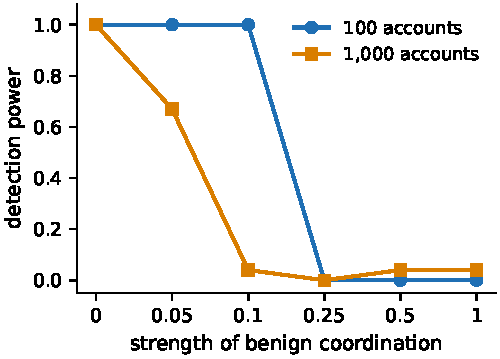
\includegraphics[width=0.6\linewidth]{figs/barrier_controlled.pdf}
\caption{The barrier in a controlled setting. Synthetic benign users with topic clusters and trends of increasing strength; campaigns of 10{,}000 extraction queries. A single tight benign cluster per window erases detection power (at strength 0.25 for 100 accounts; at 1{,}000 accounts power falls at 0.05 and vanishes at 0.1). Details in Appendix~\ref{app:controlled}.}
\label{fig:barrier}
\end{figure}

\paragraph{Sequential detection in practice.} Proposition~\ref{prop:seq} changes how to read mimicry: padding that halves a detector's weekly rate multiplies the time a defender must watch. A conformal test martingale replaces the unknown likelihood ratio, but one week can contribute only a bounded amount of evidence, so even an obvious campaign takes about three weeks to flag at $\alpha=1\%$ with our history length (Table~\ref{tab:timefrontier}).

\paragraph{The least-favourable campaign.} Proposition~\ref{prop:lfc} says the least-detectable campaign takes its on-task prompts from what real users already ask. With $p=1.48\%$, twelve weeks of 1{,}640 queries and $\alpha=1\%$, the square-root law allows about 51 extra on-task queries: against an ideal monitor that knows which accounts to watch, covert extraction is limited to the task's benign base rate. Corollary~\ref{cor:types} removes that knowledge; capacity is then counted in accounts, and the bound of about 14 posing accounts at $A=10^5$ is small because on-task users are rare ($q=0.25\%$ of benign account-weeks), not because the monitor is clever.

\takeaway{What the theory tells a provider.}{Detection is decided by the gap between a campaign and the most similar benign group, not by any signature of extraction. Measure your benign coordination; expect mimicry to cost time rather than to blind you; and expect campaigns built from real users' requests to be the hard case.}
